\chapter{Analysing Exceptions}
\label{chapter:Exceptions}
Initially it was not a goal to support exceptions, but since so many language constructs (including the magic method \inlinecode{\_\_getattr\_\_}) in Python rely so heavily on these, it became a necessity to handle these. Thus we have only concentrated on except blocks (catch blocks) without types that catches all raised exceptions. In particular we don't support except blocks like \inlinecode{except AttributeError as e}.

\section{Raising exceptions intraprocedurally}
To handle exceptions intraprocedurally our type analysis has received minor modifications\footnote{In \autoref{chap:CFGConstruction} we describe how the CFG is constructed to support exceptions}. When an exception is possibly raised the type analyser writes that particular exception object to a special fixed register where we store the latest raised exception. If the exception is raised by a \inlinecode{RaiseNode} in the CFG, the exception object will already be stored in a fixed register. This is the case because the code \inlinecode{raise Exception()} is represented as follows in our CFG:

\begin{listing}[H]
	\begin{center}
		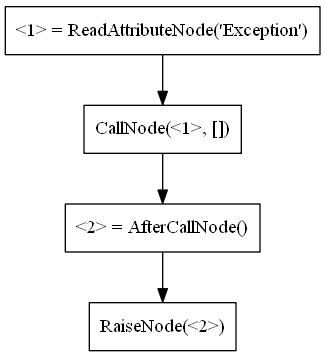
\includegraphics[width=0.4\textwidth]{images/raiseexception.png}
	\end{center}
	\vspace{-20pt}
\end{listing}

Therefore, our type analyser can just take that object (for the example: the object in \inlinecode{<2>}) and store it in the fixed register.

When an exception is not raised by a \inlinecode{RaiseNode}, our type analyser creates a new exception object. As an example of this, would be reading an absent attribute on an object. This would result in a new \inlinecode{AttributeError} object stored on the abstract heap. We do this as follows:

\begin{enumerate}
	\item The \inlinecode{\_\_builtin\_\_} module object on the heap is looked up,
	\item The attribute "AttributeError" is looked up on the \inlinecode{\_\_builtin\_\_} object from (1); this should always yield a \inlinecode{NewStyleClassObjectLabel},
	\item We manually create an instance of that particular class label found in (2), stores it on the abstract heap and finally saves it into the special fixed register.
\end{enumerate}


\section{Raising exceptions interprocedurally}
The above outline only specifies how we handle exceptions intraprocedurally, since we so far haven't specified any exception edges in our CFG going across function definitions.

We take care of exceptions interprocedurally by introducing a new type of node for function exits: \inlinecode{ExceptionalExitNode}, this new node is added to each function CFG so they now have two types of exit nodes. We now take each of the CFG nodes of the function that does not have an outgoing exception edge\footnote{If a CFG node in a function already has an outgoing exception edge, it is because it is inside a try-except block.} and connect them to the exceptional exit node with an exception edge.

Recall from \autoref{Functions} about functions, that we upon a call to a function updates the call graph with call edges from the call node to the entry node of the function, and from the exit node of the function to the after call node. To accommodate exceptions interprocedural we also add a \textit{call exception edge} from the exceptional exit node of the function to the except block of the call node. To illustrate this consider the below example together with its corresponding (partial) CFG:

\begin{listing}[H]
	\begin{minted}[linenos]{python}
class C(object):
  if (trickyComputation()):
    a = 42
x = C()
def foo():
  result = x.a
  return result
try:
  y = foo()
  z = "trickyComputation() was true"
except:
  err = "An error occured"
	\end{minted}
	\caption{An example that involves exceptions.}
	\label{code:NameExceptionExample}
\end{listing}

\begin{listing}[H]
	\begin{center}
		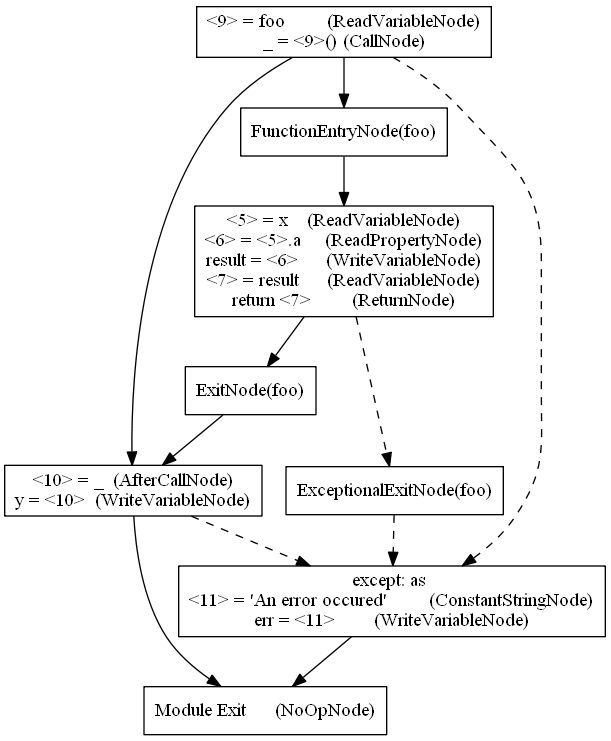
\includegraphics[width=0.75\textwidth]{images/exception1.png}
	\end{center}
	\vspace{-10pt}
\end{listing}


\section{Catching exceptions}
The constraint function for an \inlinecode{ExceptNode} in the CFG, checks the speical exception register. If the abstract value of the exception register is bottom (indicating no exceptions was raised) the solution of this node is simply set to the bottom element of the $State$ lattice. This indicates that the path is infeasible and acts as a simple sort of path sensivity. If the value of the exception register is actually poiting to an object on the abstract heap, we just clear the exception register on the stack by setting it to the bottom element of the $Value$ lattice. Now, the CFG nodes in the except block will change the solution, relatively as if an exception was raised at runtime, and the node following the try and except blocks will join the state coming from the try and except block, respectively.

Our type analyser will for \autoref{code:NameExceptionExample} conclude the following for the exit node of the program:

\begin{itemize}
	\item \inlinecode{y} is either \inlinecode{undefined} or \inlinecode{42}
	\item \inlinecode{z} is either \inlinecode{undefined} or \inlinecode{"trickyComputation() was true"}
	\item \inlinecode{err} is either \inlinecode{undefined} or \inlinecode{"An error occurred"}
\end{itemize}

For the state at the last program point in the try block, the type analyser concludes:

\begin{itemize}
	\item \inlinecode{y} is \inlinecode{undefined} or \inlinecode{42}
	\item \inlinecode{z} is \inlinecode{"trickyComputation() was true"}
\end{itemize}
